% ============================================================
% BAB 3 — DESKRIPSI SISTEM (SCOPE: DIAS) — v1
% Muhammad Dias Al Izzat — D4 TRM PENS
% Project: Sketchbook Universe
% Format: PENS Standard (A4, 12pt TNR, 1.5 spacing, 4cm/3cm margin)
% Pola: Izzah (Deskripsi Solusi → Metodologi → Desain Sistem → Jadwal)
% Post-pivot 16/6/26: nomor absen + superadmin, Top-6 check, time_spent_ms field,
%                     top6_match field, hapus Decorative category (Solid/Danger only)
% Output: 18-22 halaman DETAIL
% ============================================================

\documentclass[12pt,a4paper,oneside,openany]{report}

% ============================================================
% PACKAGES
% ============================================================
\usepackage[top=4cm,left=4cm,right=3cm,bottom=3cm]{geometry}
\usepackage{graphicx}
\usepackage{booktabs}
\usepackage{array}
\usepackage{tabularx}
\usepackage{longtable}
\usepackage{multirow}
\usepackage{float}
\usepackage{caption}
\usepackage{titlesec}
\usepackage{indentfirst}
\usepackage{setspace}
\usepackage{etoolbox}
\usepackage{fancyhdr}
\usepackage{afterpage}
\usepackage{amsmath}
\usepackage{amssymb}
\usepackage{url}
\usepackage{cite}
\usepackage{hyperref}
\hypersetup{colorlinks=false, pdfborder={0 0 0}}

% Times New Roman (pdflatex standard)
\usepackage{times}
\renewcommand{\rmdefault}{ptm}

% Line spacing 1.5
\setstretch{1.5}

% Paragraph indent (PENS standard)
\setlength{\parindent}{1.25cm}
\setlength{\parskip}{0pt}

% Chapter / Section / Subsection formatting
\titleformat{\chapter}[display]
  {\normalfont\fontsize{14pt}{16.8pt}\selectfont\bfseries\centering}
  {BAB \thechapter}
  {12pt}
  {\MakeUppercase}

\titleformat{\section}
  {\normalfont\fontsize{12pt}{14.4pt}\selectfont\bfseries}
  {\thesection}
  {1em}
  {\MakeUppercase}

\titleformat{\subsection}
  {\normalfont\fontsize{12pt}{14.4pt}\selectfont\bfseries}
  {\thesubsection}
  {1em}
  {}

\titleformat{\subsubsection}
  {\normalfont\fontsize{12pt}{14.4pt}\selectfont\bfseries\itshape}
  {\thesubsubsection}
  {1em}
  {}

\titlespacing*{\chapter}{0pt}{0pt}{24pt}
\titlespacing*{\section}{0pt}{18pt}{12pt}
\titlespacing*{\subsection}{0pt}{14pt}{8pt}

% Caption formatting (Pola Izzah)
\captionsetup[table]{font=small,labelfont=bf,name={Tabel},labelsep=period,justification=centering,aboveskip=6pt,belowskip=0pt,position=top}
\captionsetup[figure]{font=small,labelfont=bf,name={Gambar},labelsep=period,justification=centering,aboveskip=0pt,belowskip=6pt,position=bottom}

% Header / Footer (page number top-right)
\pagestyle{fancy}
\fancyhf{}
\fancyhead[R]{\thepage}
\renewcommand{\headrulewidth}{0pt}
\renewcommand{\footrulewidth}{0pt}

\fancypagestyle{plain}{
  \fancyhf{}
  \fancyhead[R]{\thepage}
  \renewcommand{\headrulewidth}{0pt}
}

% TOC formatting
\renewcommand{\contentsname}{DAFTAR ISI}
\renewcommand{\listfigurename}{DAFTAR GAMBAR}
\renewcommand{\listtablename}{DAFTAR TABEL}

% Placeholder figure helper (POLOSAN — empty box for unmade figures)
\newcommand{\placeholderfig}[2]{%
  \begin{figure}[H]
    \centering
    \fbox{\parbox{0.9\textwidth}{\centering\vspace{4cm}\textit{[Placeholder: #1 — akan dilengkapi pada tahap implementasi]}\vspace{4cm}}}
    \caption{#2}
    \label{fig:#2}
  \end{figure}
}

\begin{document}

% ============================================================
% BAB 3 — DESKRIPSI SISTEM (SCOPE: DIAS)
% ============================================================
\chapter{DESKRIPSI SISTEM}
\label{chap:bab3}

Bab ini menyajikan deskripsi solusi dan desain sistem untuk proyek \textit{Sketchbook Universe} yang berada dalam scope penulis (Dias), yaitu: Backend, REST API, Model CNN MobileNet, Penyimpanan Log SQLite, K-Means Clustering, Admin Dashboard, dan Kontrak Data Dias--Can. Modul Frontend, UI/UX, Probe UI, Animasi Momo, Level Design, dan Mekanisme HITL merupakan bagian pasangan penelitian (Can) yang dikerjakan oleh anggota tim lainnya. Bab ini disusun mengikuti urutan: deskripsi solusi, metodologi penelitian, desain sistem, pembagian tugas dan alur pengerjaan, serta jadwal penelitian. Penulis menekankan pada arsitektur backend, pipeline CNN, schema data log, endpoint REST API, algoritma K-Means, dan dashboard admin yang menjadi kontribusi inti scope penulis.

% ============================================================
\section{DESKRIPSI SOLUSI}
\label{sec:deskripsi-solusi}
% ============================================================

\textit{Sketchbook Universe} adalah simulasi interaktif berbasis web yang memfasilitasi interaksi reflektif siswa SMP terhadap output klasifikasi AI melalui mekanisme Human-in-the-Loop (HITL). Solusi ini dirancang berdasarkan empat prinsip teknis yang menjadi tanggung jawab penulis (Dias): (1) klasifikasi sketsa real-time menggunakan CNN MobileNet yang dikonversi ke TensorFlow.js untuk inferensi 100\% \textit{client-side}~\cite{ref6}\cite{ref7}\cite{ref8}; (2) pencatatan \textit{behavioral log} terstruktur via REST API Node.js/Express ke database SQLite~\cite{ref4}; (3) analisis pola keputusan siswa menggunakan K-Means clustering~\cite{ref10}\cite{ref11} untuk segmentasi tipe pengambil keputusan; dan (4) dashboard admin untuk guru/superadmin yang memvisualisasikan metrik keputusan dan hasil clustering.

Dari perspektif scope penulis, sistem memiliki lima komponen teknis utama: (1) \textbf{Model CNN MobileNet} yang dilatih pada dataset Quick Draw! dengan 116 kategori terpilih (post-RSI-1 filter --- kategori yang terlalu kompleks atau primitive dihapus) dan dikonversi ke format TensorFlow.js (\texttt{model.json} + shard files); (2) \textbf{Backend REST API} (Node.js + Express) yang menerima behavioral log dari frontend, memvalidasi payload, menyimpan ke SQLite, dan menyajikan endpoint query untuk dashboard; (3) \textbf{Database SQLite} yang menyimpan tabel \texttt{interaction\_logs}, \texttt{sessions}, \texttt{students}, \texttt{classes}, \texttt{schools}, \texttt{guru}, \texttt{clusters}, dan \texttt{users}; (4) \textbf{K-Means Worker} (Python + scikit-learn) yang menjalankan clustering offline batch pada data log terkumpul; dan (5) \textbf{Admin Dashboard} yang memvisualisasikan metrik per kelas, per siswa, dan hasil clustering.

Post-pivot 16/6/26, terdapat empat perubahan signifikan pada scope penulis: (1) \textbf{PIVOT \#1} --- penambahan aktor Superadmin dan hierarki user baru (Superadmin $\rightarrow$ Sekolah $\rightarrow$ Kelas $\rightarrow$ Siswa) mengharuskan penulis menambahkan tabel \texttt{schools}, \texttt{classes}, \texttt{guru} serta endpoint manajemen superadmin; login siswa menggunakan \texttt{class\_id + nomor\_absen} (no password), bukan gesture MediaPipe yang dideprecate; (2) \textbf{PIVOT \#2} --- mekanisme \textit{Override Budget} digantikan dengan \textbf{Top-6 Check}, sehingga backend wajib menyimpan field \texttt{top6\_match} (boolean) dan field \texttt{confidence\_top6} pada setiap log override; (3) \textbf{DECISION \#3} --- penambahan timer count-up di frontend menambahkan field \texttt{time\_spent\_ms} pada setiap event log untuk analisis durasi per aksi; (4) \textbf{DECISION \#5} --- kategori objek dipersempit menjadi Solid/Danger saja (Decorative dihapus), sehingga mapping table disederhanakan dan tabel \texttt{behavior\_mapping} tidak lagi memuat kategori Decorative.

Kontrak data antara penulis (Dias) dan rekan (Can) berpusat pada dua titik temu: (1) \textbf{Probe UI} --- tempat output AI (Top-3 + confidence dari CNN) bertemu input user (keputusan siswa dari frontend); (2) \textbf{Endpoint \texttt{POST /api/logs/event}} --- tempat frontend mengirim behavioral log ke backend. Kontrak data lengkap diuraikan pada Sub-bab~\ref{subsec:kontrak-data}. Selain menerima log, penulis juga menyediakan model CNN MobileNet yang telah dikonversi ke TensorFlow.js sebagai aset statis yang diload oleh browser siswa saat aplikasi dibuka. Kontrak data ini memastikan bahwa rekan tidak perlu memahami detail training model, dan penulis tidak perlu memahami detail interaksi gameplay.

% ============================================================
\section{METODOLOGI PENELITIAN}
\label{sec:metodologi-penelitian}
% ============================================================

Metodologi penelitian menjelaskan pendekatan, metode pengembangan, analisis masalah, teknik pengumpulan dan analisis data, serta metode pengujian yang digunakan dalam proyek ini. Pendekatan penelitian bersifat \textit{mixed methods} dengan paradigma \textit{Research and Development} (R\&D). Metode pengembangan perangkat lunak mengikuti model \textit{Waterfall SDLC} dengan lima tahap berurutan. Analisis masalah dilakukan menggunakan diagram Fishbone (Ishikawa) dengan pendekatan 6M untuk mengidentifikasi \textit{root cause} dari \textit{automation bias} pada siswa SMP terhadap output AI. Pengumpulan data dilakukan melalui \textit{behavioral log} sistem (yang dikirim ke backend penulis), akurasi model CNN via confusion matrix, dan kuesioner System Usability Scale (SUS) yang di-share dengan rekan. Analisis data menggunakan K-Means clustering untuk segmentasi pola perilaku siswa dan statistik deskriptif untuk akurasi model. Pengujian dilakukan dengan black-box testing, akurasi model (confusion matrix), dan SUS untuk dashboard admin.

\subsection{Pendekatan dan Jenis Penelitian}
\label{subsec:pendekatan-penelitian}

Penelitian ini menggunakan pendekatan \textit{mixed methods}~\cite{ref13} yang menggabungkan data kuantitatif (akurasi model CNN, behavioral log, skor SUS, metrik clustering) dan data kualitatif (interpretasi cluster, profil perilaku siswa per cluster). Pemilihan \textit{mixed methods} didasarkan pada karakteristik proyek yang mengukur performa teknis model (kuantitatif) sekaligus menginterpretasikan pola perilaku siswa hasil clustering (kualitatif). Creswell~\cite{ref13} menegaskan bahwa \textit{mixed methods} cocok untuk penelitian yang membutuhkan triangulasi data dari multiple sources.

Jenis penelitian ini adalah \textit{Research and Development} (R\&D)~\cite{ref12}, yaitu penelitian yang menghasilkan produk berupa sistem perangkat lunak (\textit{Sketchbook Universe} bagian backend, CNN, dan analisis) beserta dokumentasi akademis. Sugiyono~\cite{ref12} mendefinisikan R\&D sebagai metode penelitian yang digunakan untuk menghasilkan produk tertentu dan menguji keefektifan produk tersebut. Dalam konteks penulis, produk yang dikembangkan adalah model CNN MobileNet yang dikonversi ke TF.js, backend REST API dengan SQLite, pipeline K-Means clustering, dan admin dashboard yang diuji melalui confusion matrix, black-box testing, dan SUS.

\subsection{Metode Pengembangan (Waterfall SDLC)}
\label{subsec:metode-pengembangan}

Metode pengembangan perangkat lunak yang digunakan adalah \textit{Waterfall SDLC}~\cite{ref9}\cite{ref10} dengan lima tahap berurutan: (1) Analisis Kebutuhan, (2) Perancangan Sistem, (3) Implementasi, (4) Integrasi dan Pengujian, dan (5) Pemeliharaan dan Dokumentasi. Pemilihan Waterfall didasarkan pada karakteristik proyek yang memiliki scope jelas, tim kecil (dua orang: Can dan Dias), serta kebutuhan dokumentasi akademis yang mensyaratkan setiap tahap terdefinisi secara eksplisit. Pressman~\cite{ref9} menegaskan bahwa Waterfall cocok untuk proyek dengan kebutuhan yang stabil dan tim yang dapat berkomitmen pada satu paradigma desain dari awal.

Gambar~\ref{fig:waterfall-sdlc} menunjukkan diagram alur Waterfall SDLC yang diadaptasi untuk proyek \textit{Sketchbook Universe}. Setiap tahap menghasilkan \textit{deliverable} yang menjadi input bagi tahap berikutnya.

% Mermaid source (POLOSAN, no classDef/style):
% flowchart TD
%     A["Analisis Kebutuhan"] --> B["Perancangan Sistem"]
%     B --> C["Implementasi"]
%     C --> D["Integrasi & Pengujian"]
%     D --> E["Pemeliharaan & Dokumentasi"]
\placeholderfig{Gambar Waterfall SDLC --- 5 Tahap Berurutan}{Gambar 3.1 Metode Pengembangan Waterfall SDLC untuk Sketchbook Universe}

Kelima tahap Waterfall diadaptasi untuk scope penulis (Dias) sebagai berikut:

\textbf{Tahap 1 --- Analisis Kebutuhan.} Tahap ini mengidentifikasi kebutuhan backend: kebutuhan data log (Tabel~\ref{tab:json-log}), endpoint REST API (Tabel~\ref{tab:api-endpoints}), schema database, model CNN MobileNet (Tabel~\ref{tab:hyperparameter}), dan algoritma K-Means (Tabel~\ref{tab:kmeans-feature}). Output tahap ini meliputi dokumen kontrak data Can-Dias dan spesifikasi teknis backend.

\textbf{Tahap 2 --- Perancangan Sistem.} Tahap ini menerjemahkan kebutuhan menjadi desain konkret: arsitektur sistem hybrid (browser inference + server-side services), perancangan model CNN, perancangan data log schema, perancangan backend API, perancangan K-Means clustering, perancangan admin dashboard, dan perancangan kontrak data. Output tahap ini meliputi seluruh sub-bab Desain Sistem (Sub-bab~\ref{subsec:sistem-global}--\ref{subsec:kontrak-data}).

\textbf{Tahap 3 --- Implementasi.} Tahap ini mengodekan desain menjadi sistem yang berjalan. Scope penulis (Dias) mencakup: training CNN MobileNet di Python/TensorFlow, konversi model ke TF.js, implementasi backend Node.js/Express, schema dan migrasi SQLite, K-Means worker Python, dan admin dashboard web.

\textbf{Tahap 4 --- Integrasi dan Pengujian.} Tahap ini mengintegrasikan modul backend (scope penulis) dengan modul frontend (scope rekan Can) dan melakukan pengujian black-box, akurasi model via confusion matrix, dan SUS untuk dashboard admin. Titik integrasi utama adalah endpoint \texttt{POST /api/logs/event} dan \texttt{POST /probe/override} (Top-6 Check).

\textbf{Tahap 5 --- Pemeliharaan dan Dokumentasi.} Tahap ini meliputi perbaikan bug yang ditemukan selama pengujian, optimasi model (quantization bila ukuran $>$ 5 MB), penulisan laporan akhir, dan dokumentasi kode sumber.

\subsection{Analisis Masalah (Fishbone 6M)}
\label{subsec:analisis-masalah}

Analisis masalah menggunakan diagram Fishbone (Ishikawa)~\cite{ref14} dengan pendekatan 6M untuk mengidentifikasi \textit{root cause} dari permasalahan inti penelitian: \textbf{automation bias pada siswa SMP terhadap output AI}. Ishikawa~\cite{ref14} memperkenalkan diagram Fishbone sebagai alat analisis \textit{root cause} yang mengkategorikan faktor-faktor penyebab ke dalam enam dimensi (6M): \textit{Man}, \textit{Method}, \textit{Machine}, \textit{Material}, \textit{Measurement}, dan \textit{Environment}. Dari perspektif scope penulis (backend, CNN, K-Means), analisis 6M menekankan pada faktor teknis yang dapat diatasi melalui komponen backend.

Tabel~\ref{tab:fishbone-6m} merinci keenam dimensi 6M beserta sub-cause yang teridentifikasi dan implikasi desain pada scope penulis.

\begin{table}[H]
\centering
\caption{Analisis Masalah Automation Bias --- Fishbone 6M (Perspektif Scope Dias)}
\label{tab:fishbone-6m}
\begin{tabular}{|p{2.5cm}|p{5cm}|p{6cm}|}
\hline
\textbf{Dimensi 6M} & \textbf{Sub-Cause Teridentifikasi} & \textbf{Implikasi Desain (Scope Dias)} \\ \hline
Man (Manusia) & (1) Guru belum punya alat observasi pola keputusan siswa; (2) Peneliti belum punya dataset perilaku siswa terhadap AI klasifikasi sketsa; (3) Superadmin manual untuk multi-school deployment tidak scalable & Admin dashboard dengan decision distribution + K-Means cluster; behavioral log schema terstruktur; superadmin UI + endpoints untuk provisioning multi-school \\ \hline
Method (Metode) & (1) Tidak ada mekanisme anti-cheat untuk override siswa; (2) Tidak ada segmentasi tipe pengambil keputusan siswa; (3) Pembelajaran AI di SMP masih konseptual & Top-6 Check mechanism (backend verify); K-Means clustering dengan feature engineering per siswa; dataset behavioral log terstruktur \\ \hline
Machine (Mesin) & (1) Model CNN MobileNet memiliki confidence calibration belum sempurna; (2) Inferensi server-side memiliki latensi 200--500 ms; (3) Browser siswa heterogen & Training MobileNet V2 dengan transfer learning; inferensi 100\% client-side via TF.js (15--100 ms); quantization model untuk loading cepat \\ \hline
Material (Materi) & (1) Dataset Quick Draw! terlalu luas (ratusan kategori); (2) Tidak ada dataset behavioral log siswa SMP terhadap AI; (3) Tidak ada lookup table perilaku objek untuk gameplay & Kurasi 116 kategori post-RSI-1 (medium difficulty); SQLite database interaction\_logs; lookup table Solid/Danger (Decorative dihapus) \\ \hline
Measurement (Pengukuran) & (1) Tidak ada metrik standar untuk automation bias SMP; (2) Decision latency dan top6\_match belum terdefinisi sebagai metrik; (3) Akurasi model belum dievaluasi via confusion matrix & Metrik: decision type distribution, time\_spent\_ms, top6\_match\_rate; confusion matrix untuk CNN (akurasi, precision, recall, F1); SUS untuk dashboard admin \\ \hline
Environment (Lingkungan) & (1) Bandwidth sekolah terbatas untuk streaming inferensi; (2) Device kelas berbagi, data harus terpisah antar sekolah; (3) Browser siswa heterogen & Inferensi 100\% client-side (offline setelah model diload); isolasi data antar sekolah (UU PDP No. 27/2022); model di-cache di browser siswa; SQLite embedded (no server DB setup) \\ \hline
\end{tabular}
\end{table}

Diagram Fishbone 6M lengkap ditunjukkan pada Gambar~\ref{fig:fishbone-6m}. Diagram menampilkan \textit{root cause} (automation bias pada siswa SMP) di sisi kanan, dengan enam cabang utama 6M yang masing-masing memiliki 2--3 sub-cause.

% Mermaid source (POLOSAN, no classDef/style) tersedia di:
% ../../diagrams/generated_sketchbook_universe/fishbone_6m.mmd
% Render ke PNG via: mmdc -i fishbone_6m.mmd -o fishbone_6m.png -b white -w 1600 -H 900
% Output PNG: ../../diagrams/generated_sketchbook_universe/fishbone_6m.png
\begin{figure}[H]
    \centering
    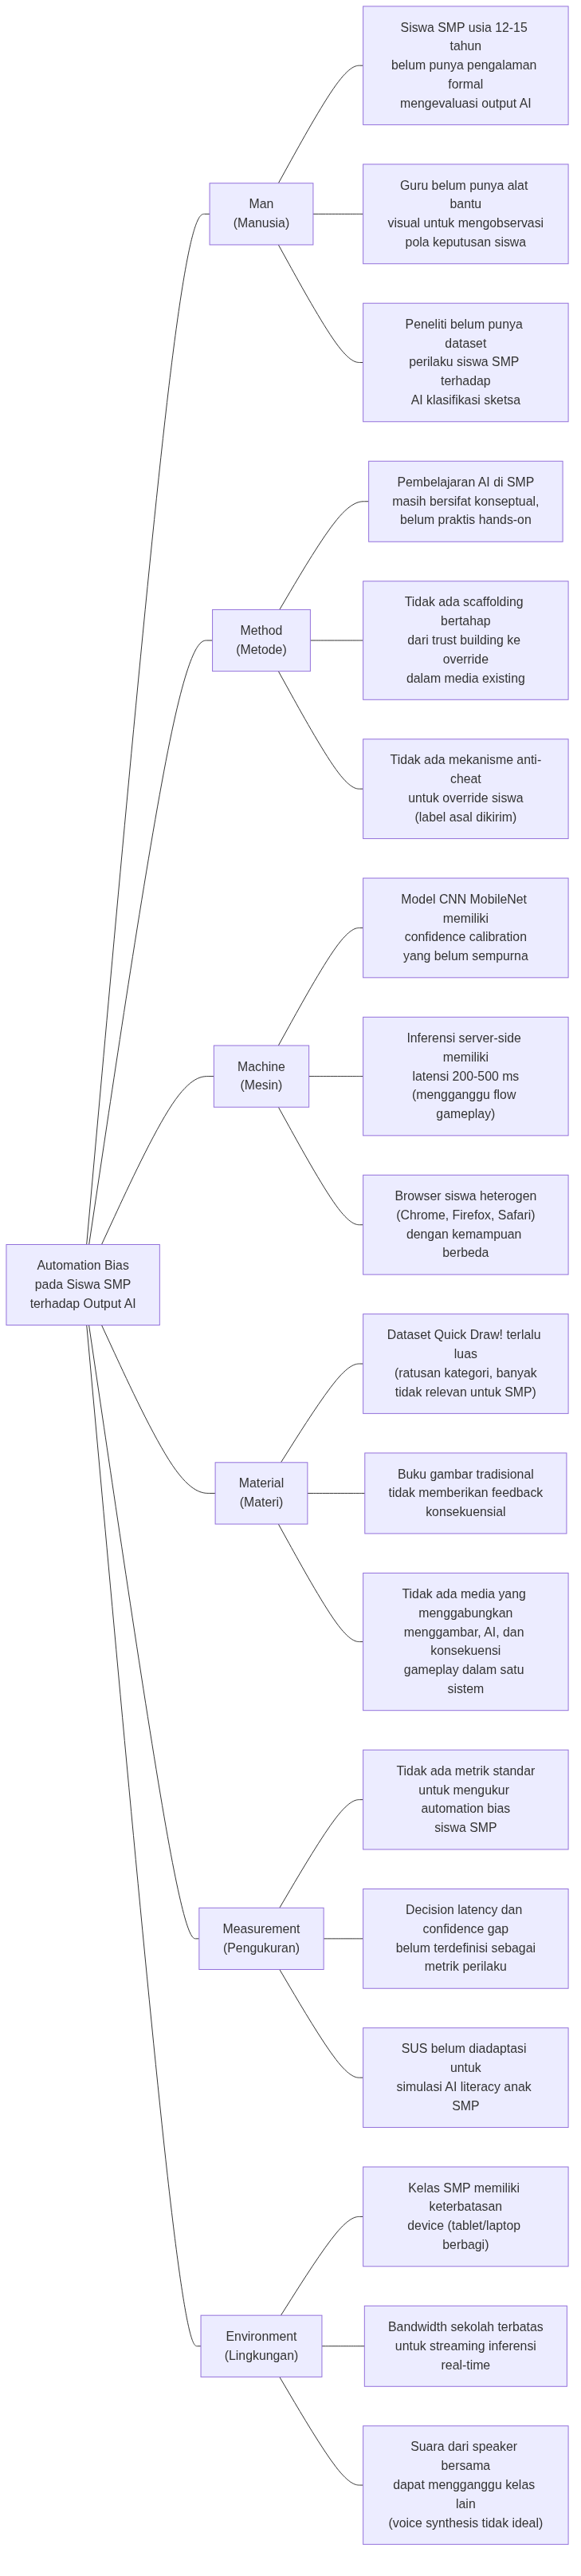
\includegraphics[width=0.85\textwidth]{../../diagrams/generated_sketchbook_universe/fishbone_6m.png}
    \caption{Fishbone Diagram 6M untuk Analisis Root Cause Automation Bias pada Siswa SMP}
    \label{fig:fishbone-6m}
\end{figure}

Diagram Fishbone 6M selengkapnya juga tersedia dalam format Mermaid POLOSAN di file \texttt{fishbone\_6m.mmd} (dirender terpisah ke PNG).

\subsection{Teknik Pengumpulan Data}
\label{subsec:teknik-pengumpulan-data}

Pengumpulan data dilakukan melalui tiga teknik yang menjadi tanggung jawab scope penulis:

\textbf{(1) Behavioral Log via REST API.} Frontend Can mengirim setiap aksi siswa (draw, accept, correct, override, complete\_level, fail\_level) ke endpoint \texttt{POST /api/logs/event} (fire-and-forget pattern). Backend penulis menerima, memvalidasi, dan menyimpan ke tabel \texttt{interaction\_logs} di SQLite. Setiap log memuat field baru post-pivot 16/6/26: \texttt{time\_spent\_ms} (durasi per aksi, dari timer count-up frontend), \texttt{top6\_match} (boolean hasil Top-6 Check untuk override), dan \texttt{confidence\_top6} (confidence tertinggi dari Top-6 prediksi). Log ini merupakan sumber data utama untuk K-Means clustering dan dashboard guru.

\textbf{(2) Confusion Matrix untuk Model CNN.} Setelah training CNN MobileNet pada dataset Quick Draw! (116 kategori post-RSI-1), model dievaluasi menggunakan confusion matrix pada test set (20\% dari dataset). Metrik yang diukur: akurasi global, precision per kategori, recall per kategori, dan F1-score per kategori. Target akurasi $\geq 85\%$ pada test set. Confusion matrix juga digunakan untuk mengidentifikasi kategori yang sering tertukar (mis: ladder vs fence) sebagai input untuk desain level (Level~2 ambiguity).

\textbf{(3) SUS untuk Admin Dashboard.} Setelah admin dashboard selesai, 2--3 guru mengisi kuesioner SUS~\cite{ref15}\cite{ref16} untuk mengevaluasi usability dashboard. SUS dilakukan terpisah dari SUS frontend Can (yang ditujukan untuk siswa) karena target user berbeda (guru vs siswa). Target skor SUS dashboard $\geq 68$.

\subsection{Teknik Analisis Data}
\label{subsec:teknik-analisis-data}

Analisis data menggunakan dua teknik komplementer:

\textbf{(1) K-Means Clustering untuk Behavioral Log.} Behavioral log yang terkumpul di-feature engineering menjadi matriks fitur per siswa. Fitur yang diekstrak: \texttt{accept\_rate}, \texttt{correct\_rate}, \texttt{override\_rate}, \texttt{mean\_latency\_ms} (dari \texttt{time\_spent\_ms}), \texttt{confidence\_gap\_mean}, \texttt{override\_frequency}, dan \texttt{top6\_match\_rate} (rasio override yang diterima via Top-6 Check). Fitur dinormalisasi (z-score normalization) lalu di-cluster menggunakan K-Means. Jumlah cluster $k$ ditentukan via elbow method dan silhouette score, kandidat $k = 3$--$5$. Hasil clustering menghasilkan segmentasi tipe pengambil keputusan siswa, misalnya: \textit{Cluster 1 --- Tipe Pasif (Automation Bias Prone)}, \textit{Cluster 2 --- Tipe Evaluatif (Calibrated Evaluator)}, \textit{Cluster 3 --- Tipe Kritis (Overconfident Override)}. Detail teknis K-Means diuraikan pada Sub-bab~\ref{subsec:kmeans-clustering}.

\textbf{(2) Statistik Deskriptif untuk Akurasi Model.} Akurasi, precision, recall, dan F1-score dihitung dari confusion matrix. Persamaan~\ref{eq:accuracy}--\ref{eq:f1} merumuskan keempat metrik tersebut.

\begin{equation}
\label{eq:accuracy}
\text{Accuracy} = \frac{TP + TN}{TP + TN + FP + FN}
\end{equation}

\begin{equation}
\label{eq:precision}
\text{Precision} = \frac{TP}{TP + FP}
\end{equation}

\begin{equation}
\label{eq:recall}
\text{Recall} = \frac{TP}{TP + FN}
\end{equation}

\begin{equation}
\label{eq:f1}
F1 = 2 \times \frac{\text{Precision} \times \text{Recall}}{\text{Precision} + \text{Recall}}
\end{equation}

\subsection{Metode Pengujian}
\label{subsec:metode-pengujian}

Pengujian sistem dilakukan dengan tiga metode:

\textbf{(1) Black-Box Testing untuk Backend API.} Pengujian fungsionalitas endpoint REST API dari perspektif input-output. Skenario mencakup: \texttt{POST /auth/login} (valid/invalid nomor absen), \texttt{POST /logs/event} (validasi payload), \texttt{POST /probe/override} dengan Top-6 Check (match/no-match), \texttt{POST /analysis/trigger-kmeans}, \texttt{GET /analysis/clusters/\{class\_id\}}, dan endpoint superadmin (Create School, Create Class, Generate Nomor Absen, Create Guru, Assign Guru to Class). Setiap skenario memiliki \textit{expected output} yang didefinisikan sebelum pengujian.

\textbf{(2) Akurasi Model via Confusion Matrix.} Model CNN MobileNet dievaluasi pada test set dengan confusion matrix. Selain akurasi global, diukur precision, recall, dan F1-score per kategori. Kategori dengan F1-score rendah ($<$ 0.70) diidentifikasi untuk iterasi training (data augmentation tambahan, hyperparameter tuning, atau penggantian kategori bila tidak dapat diperbaiki).

\textbf{(3) SUS untuk Admin Dashboard.} Pengujian usability dashboard dari perspektif guru (target user dashboard). SUS dilakukan dengan 2--3 guru yang mencoba fitur dashboard: View Class Dashboard, View Individual Student History, Trigger K-Means Analysis, View Cluster Distribution, Export Class Data. Target skor SUS $\geq 68$ (above average menurut Bangor et al.~\cite{ref16}).

% ============================================================
\section{DESAIN SISTEM}
\label{sec:desain-sistem}
% ============================================================

Desain sistem menguraikan keputusan desain yang diambil berdasarkan prinsip-prinsip akademis dari Bab~2 dan hasil analisis Fishbone 6M pada Sub-bab~\ref{subsec:analisis-masalah}. Setiap keputusan desain disertai dengan justifikasi teknis agar hubungan antara teori dan implementasi dapat ditelusuri secara eksplisit. Desain sistem meliputi: perancangan sistem global, arsitektur sistem, model CNN MobileNet, use case, data log schema, backend API, K-Means clustering, admin dashboard, sequence diagram, klasifikasi objek, technology stack, dan kontrak data Dias--Can.

\subsection{Perancangan Sistem Global}
\label{subsec:sistem-global}

Desain sistem global menggunakan model Input--Process--Output (IPO) yang terbagi menjadi empat layer proses: \textit{Interactive Simulation Layer}, \textit{AI Classification Layer}, \textit{Decision \& Consequence Layer}, dan \textit{Data \& Analysis Layer}. Pembagian ini menunjukkan bahwa sistem terdiri dari blok fungsi utama yang saling terhubung, bukan satu flow panjang tanpa struktur.

\textbf{Input} berisi semua hal yang masuk ke sistem dari sisi user dan konteks permainan. Siswa memilih class\_id dan nomor absen untuk login, menggambar objek di canvas, mengambil keputusan terhadap prediksi AI (Accept/Correct/Override), dan bermain di level tertentu. Post-pivot 16/6/26, login menggunakan nomor absen alih-alih gesture MediaPipe.

\textit{Interactive Simulation Layer} adalah bagian yang membuat siswa masuk ke pengalaman sistem. Di sini ada onboarding, drawing canvas, Probe UI, gameplay 2D, dan feedback Momo. Layer ini dominan scope rekan (Can).

\textit{AI Classification Layer} adalah bagian yang membaca gambar user. Gambar dari canvas masuk ke preprocessing, lalu diprediksi oleh CNN MobileNet di TensorFlow.js (client-side inference), kemudian menghasilkan Top-6 predictions dan confidence scores. Top-3 ditampilkan ke siswa (transparent), Top-4 s/d Top-6 disimpan internal untuk Top-6 Check (rahasia). Layer ini merupakan kontribusi scope penulis --- training dan konversi model --- yang dijalankan di browser siswa.

\textit{Decision \& Consequence Layer} adalah jembatan antara AI dan game. Setelah AI memberi prediksi, sistem tidak langsung menjalankan hasil AI. User masuk lewat Probe UI, lalu keputusan akhirnya menjadi final label. Final label itu baru dipetakan menjadi Solid atau Danger (Decorative dihapus post-pivot DECISION \#5). Override memicu Top-6 Check di backend yang memutuskan auto-accept atau force redraw.

\textit{Data \& Analysis Layer} menerima log dari proses interaksi dan gameplay. Data dikirim via REST API ke backend, disimpan di SQLite, lalu diproses untuk analisis pola keputusan. K-Means clustering dijalankan di server menggunakan Python (scikit-learn). Dashboard guru memvisualisasikan hasil analisis. Layer ini dominan scope penulis.

\textbf{Catatan penulis:} Gambar diagram IPO Global akan dibuat manual oleh penulis pada tahap implementasi menggunakan draw.io atau Figma.

\placeholderfig{Gambar Desain Sistem Global IPO --- 4 Layer}{Gambar 3.3 Desain Sistem Global Input Process Output 4 Layer Sketchbook Universe}

\subsection{Perancangan Arsitektur Sistem Hybrid}
\label{subsec:arsitektur}

Proyek ini mengadopsi pola \textit{Hybrid Architecture} yang menggabungkan \textit{Browser-Based Inference} untuk klasifikasi AI dan \textit{Server-Side Services} untuk layanan pendukung. Inferensi CNN MobileNet berjalan sepenuhnya di browser siswa menggunakan TensorFlow.js, sehingga data gambar siswa tidak pernah keluar dari perangkat mereka. Di sisi lain, server backend (Node.js/Express + SQLite) menangani layanan yang memerlukan persistensi, autentikasi, analisis, dan visualisasi --- termasuk REST API logging, JWT authentication untuk dashboard guru, K-Means clustering, dan ekspor data.

Pemisahan ini bukan arbitrer. Inferensi dikategorikan client-side karena dua alasan: (1) privasi data siswa --- gambar tidak keluar device, sesuai COPPA/GDPR-K; (2) latensi rendah (15--100 ms vs 200--500 ms jika lewat server). Layanan pendukung dikategorikan server-side karena memerlukan persistensi data lintas sesi, akses terpusat oleh guru, dan komputasi analisis yang tidak perlu real-time di browser siswa.

Dari sisi penulis (scope Dias), arsitektur backend terdiri dari komponen-komponen berikut:

\textbf{(1) REST API (Node.js/Express).} Endpoint utama meliputi \texttt{POST /api/logs/event} untuk menerima log dari frontend, \texttt{POST /probe/override} untuk Top-6 Check, \texttt{GET /api/sessions} untuk mengambil daftar sesi, \texttt{GET /api/sessions/:id/metrics} untuk mengambil metrik keputusan, \texttt{GET /api/export/csv} dan \texttt{GET /api/export/json} untuk ekspor data. Endpoint superadmin (post-pivot 16/6/26) meliputi \texttt{POST /api/superadmin/schools}, \texttt{POST /api/superadmin/classes}, \texttt{POST /api/superadmin/students/generate}, \texttt{POST /api/superadmin/guru}, \texttt{POST /api/superadmin/assign-guru}. API menggunakan JWT authentication untuk melindungi akses dashboard guru dan superadmin.

\textbf{(2) SQLite Database.} Menyimpan interaction log, session data, students, classes, schools, guru, users, dan clusters. SQLite dipilih karena ringan, tanpa konfigurasi server tambahan, dan cukup untuk skala data penelitian (puluhan siswa, bukan ribuan).

\textbf{(3) K-Means Clustering (Python/scikit-learn).} Menerima data log yang telah di-feature engineering, menjalankan K-Means clustering untuk mengelompokkan tipe pengambil keputusan siswa, dan menghasilkan label cluster. Python dipilih karena scikit-learn menyediakan implementasi K-Means yang matang dan interoperabilitas dengan pandas untuk feature engineering.

\textbf{(4) Admin Dashboard.} Panel web yang memvisualisasikan metrik keputusan siswa dan hasil clustering. Dashboard mengakses data melalui REST API yang sama, sehingga guru tidak perlu akses langsung ke database.

\textbf{(5) Model File Serving.} Server menyajikan aset model TensorFlow.js (\texttt{model.json} + shard files) sebagai file statis. Model diload oleh browser siswa saat pertama kali membuka aplikasi, lalu di-cache untuk sesi berikutnya. Server tidak menjalankan inference --- ia hanya menyediakan file model.

\textbf{Catatan penulis:} Gambar diagram arsitektur akan dibuat manual oleh penulis pada tahap implementasi.

\placeholderfig{Gambar Arsitektur Sistem Hybrid --- Browser Inference + Server Services}{Gambar 3.4 Arsitektur Sistem Hybrid Browser-Based Inference dan Server-Side Services}

\subsection{Perancangan Model CNN MobileNet}
\label{subsec:cnn-model}

Model klasifikasi gambar menggunakan arsitektur CNN MobileNet V2 sebagai \textit{backbone}. MobileNet dipilih karena dirancang untuk perangkat dengan resource terbatas --- termasuk browser --- tanpa mengorbankan akurasi secara signifikan~\cite{ref6}. Model dilatih menggunakan dataset Quick Draw! dari Google~\cite{ref7} dengan 116 kategori terpilih (post-RSI-1 filter).

\subsubsection{Pemilihan Kategori Dataset (116 Kategori Post-RSI-1)}

Dari ratusan kategori yang tersedia di Quick Draw!, dipilih 116 kategori yang memenuhi kriteria RSI-1 (post-pivot 16/6/26): (1) bukan geometric primitive (line, circle, square, triangle --- dihapus total); (2) bukan hewan (cat, dog, elephant, dll --- dihapus untuk menghindari confusion matrix antar hewan); (3) bukan landmark/kompleks ekstrem (Eiffel Tower, Mona Lisa, Great Wall --- dihapus); (4) bukan single-stroke (smiley face, eye, dot --- dihapus). Yang dipertahankan: everyday objects (clock, cup, hat, key, umbrella), simple food (apple, donut, pizza slice), nature (sun, moon, star, tree, flower, cloud), dan basic vehicles (car, bus, bicycle) --- semua dengan stroke 4--15.

Setiap kategori harus dapat dipetakan ke salah satu dari dua behavior (Solid atau Danger; Decorative dihapus post-pivot DECISION \#5) dan memiliki minimal 50.000 sampel di Quick Draw! untuk training. Contoh kategori Solid: ladder, bridge, chair, table, plank. Contoh kategori Danger: knife, sword, axe, duri (thorns --- bukan pisau, sesuai arahan Bu Hesti). Pemilihan kategori ini memastikan bahwa setiap level bisa menghasilkan confidence range yang berbeda secara programatik.

\subsubsection{Arsitektur Model (MobileNet V2 + Transfer Learning)}

Model menggunakan MobileNet V2 sebagai feature extractor, dengan layer klasifikasi kustom di atasnya. Input berupa gambar grayscale 28$\times$28 piksel (sesuai format Quick Draw!). Preprocessing meliputi: resize, normalisasi (0--1), konversi grayscale ke RGB 3-channel (kompatibilitas dengan MobileNet V2 input shape), dan konversi ke tensor. Output berupa probabilitas untuk 116 kategori menggunakan softmax.

Hyperparameter awal ditunjukkan pada Tabel~\ref{tab:hyperparameter}.

\begin{table}[H]
\centering
\caption{Hyperparameter CNN MobileNet V2 --- Initial Value}
\label{tab:hyperparameter}
\begin{tabular}{|l|l|}
\hline
\textbf{Hyperparameter} & \textbf{Nilai Awal} \\ \hline
Feature Extractor & MobileNet V2 (pre-trained ImageNet) \\ \hline
Epoch & 100 \\ \hline
Learning Rate & 0.001 \\ \hline
Optimizer & Adam \\ \hline
Loss Function & Categorical crossentropy \\ \hline
Batch Size & 32 \\ \hline
Data Augmentation & Rotasi $\pm$15$^\circ$, flip horizontal, zoom $\pm$10\% \\ \hline
Train/Test Split & 80/20 \\ \hline
Target Akurasi & $\geq$ 85\% pada test set \\ \hline
\end{tabular}
\end{table}

Nilai hyperparameter bersifat fleksibel dan dapat disesuaikan berdasarkan hasil evaluasi performa model pada data uji. Bila akurasi belum mencapai target 85\%, dilakukan iterasi: (1) tambah data augmentation, (2) tune learning rate (0.0005 atau 0.0001), (3) unfreeze beberapa layer MobileNet V2 untuk fine-tuning, (4) ganti kategori dengan F1-score rendah.

\subsubsection{Konversi ke TensorFlow.js}

Setelah model mencapai akurasi yang memadai ($\geq 85\%$), model dikonversi dari format Keras (\texttt{.h5}) ke format TensorFlow.js menggunakan \texttt{tensorflowjs\_converter}. Konversi menghasilkan file \texttt{model.json} (metadata model) dan shard files (bobot model). File-file ini disajikan sebagai aset statis oleh server dan diload oleh browser siswa saat aplikasi dibuka.

Target ukuran model setelah konversi adalah $<$ 5 MB agar loading time di browser tetap cepat. Jika ukuran melebihi target, dilakukan quantization (float16 atau int8) untuk mengurangi ukuran file. Smilkov et al.~\cite{ref8} menegaskan bahwa TF.js memungkinkan inferensi CNN di browser dengan latency 15--100 ms untuk model berukuran $<$ 5 MB, sehingga inferensi real-time di gameplay dapat berjalan tanpa blocking.

\placeholderfig{Gambar Arsitektur CNN MobileNet V2 --- Training ke TF.js Export}{Gambar 3.5 Arsitektur CNN MobileNet V2 dari Training ke Konversi TensorFlow.js}

\subsection{Perancangan Use Case}
\label{subsec:use-case}

Use case diagram memetakan aktor eksternal dan tujuan utama sistem. Post-pivot 16/6/26 (PIVOT \#1), terdapat tiga aktor utama: Siswa, Guru/Admin Sekolah, dan Superadmin. Aktor Superadmin merupakan aktor baru yang ditambahkan untuk mendukung deployment multi-sekolah dan pengelolaan nomor absen siswa per kelas. Sistem memiliki total 30 use case (UC-01 s/d UC-30) yang terdistribusi pada tiga aktor. Daftar lengkap 30 use case beserta deskripsinya telah diuraikan pada Bab~3 Can (Sub-bab Use Case Sistem) karena bersifat shared --- kedua proposal merujuk pada use case yang sama. Tabel~\ref{tab:use-case-dias-focus} merangkum use case yang berada di tanggung jawab scope penulis (Dias).

\begin{table}[H]
\centering
\caption{Use Case yang Menjadi Tanggung Jawab Scope Dias}
\label{tab:use-case-dias-focus}
\begin{tabular}{|p{1cm}|p{4cm}|p{2.5cm}|p{6cm}|}
\hline
\textbf{ID} & \textbf{Nama Use Case} & \textbf{Aktor} & \textbf{Implikasi Backend (Scope Dias)} \\ \hline
UC-05 & Generate Nomor Absen Siswa & Superadmin & Endpoint \texttt{POST /api/superadmin/students/generate}, INSERT N slot siswa kosong \\ \hline
UC-06 & Create Guru Account & Superadmin & Endpoint \texttt{POST /api/superadmin/guru}, hash password bcrypt \\ \hline
UC-07 & Assign Guru to Class & Superadmin & Endpoint \texttt{POST /api/superadmin/assign-guru}, mapping guru\_class \\ \hline
UC-12 & Login Guru & Guru & Endpoint \texttt{POST /api/auth/login/guru}, JWT generation \\ \hline
UC-14 & View Class Dashboard & Guru & Endpoint \texttt{GET /api/dashboard/\{class\_id\}}, agregasi metrik per kelas \\ \hline
UC-15 & View Individual Student History & Guru & Endpoint \texttt{GET /api/students/\{student\_id\}/history} \\ \hline
UC-16 & Export Class Data & Guru & Endpoint \texttt{GET /api/export/csv} dan \texttt{/api/export/json} \\ \hline
UC-17 & Trigger K-Means Analysis & Guru & Endpoint \texttt{POST /api/analysis/trigger-kmeans}, submit job ke K-Means Worker \\ \hline
UC-18 & View Cluster Distribution & Guru & Endpoint \texttt{GET /api/analysis/clusters/\{class\_id\}} \\ \hline
UC-21 & Login Nomor Absen & Siswa & Endpoint \texttt{POST /api/auth/login}, no password, JWT 4 jam expiry \\ \hline
UC-28 & Override Prediction & Siswa & Endpoint \texttt{POST /probe/override}, Top-6 Check di backend \\ \hline
\end{tabular}
\end{table}

Use case yang bersifat frontend-only (UC-22 View Onboarding, UC-23 Start Level, UC-24 Draw Object, UC-25 View AI Prediction, UC-26 Accept, UC-27 Correct, UC-29 Top-6 Verification Result, UC-30 View Personal History) berada di tanggung jawab rekan (Can). Namun, use case UC-24, UC-26, UC-27, dan UC-28 menghasilkan behavioral log yang dikirim ke backend penulis via \texttt{POST /api/logs/event}, sehingga penulis wajib menyediakan endpoint penerima dan schema penyimpanan yang sesuai.

\subsection{Perancangan Data Log Schema}
\label{subsec:data-log-schema}

Log interaksi menyimpan data utama dari momen Human-in-the-Loop: prediksi AI, confidence, keputusan siswa, final label, behavior objek, hasil gameplay, waktu keputusan, dan hasil Top-6 Check. Schema ini dirancang untuk mendukung analisis pola keputusan dan K-Means clustering. Tabel~\ref{tab:json-log} merinci struktur JSON interaction log yang dikirim dari frontend ke backend.

\begin{table}[H]
\centering
\caption{Struktur JSON Interaction Log (Post-Pivot 16/6/26)}
\label{tab:json-log}
\begin{tabular}{|p{3.5cm}|p{2.5cm}|p{7cm}|}
\hline
\textbf{Field} & \textbf{Tipe} & \textbf{Deskripsi} \\ \hline
\texttt{session\_token} & String (JWT) & Token sesi siswa, validasi via \texttt{POST /api/auth/login} \\ \hline
\texttt{student\_id} & Integer & ID siswa (di-derive dari session\_token di backend) \\ \hline
\texttt{class\_id} & Integer & ID kelas siswa \\ \hline
\texttt{school\_id} & Integer & ID sekolah siswa (untuk isolasi data) \\ \hline
\texttt{level} & Integer & Level permainan (1, 2, 3) \\ \hline
\texttt{probe\_id} & String & ID unik per momen Probe UI \\ \hline
\texttt{event\_type} & String & Jenis event: draw\_start, draw\_end, accept, correct, override, move\_stickman, complete\_level, fail\_level \\ \hline
\texttt{decision\_type} & String (nullable) & Accept / Correct / Override (hanya untuk event accept/correct/override) \\ \hline
\texttt{top3\_predictions} & Array[String] & Tiga prediksi teratas dari CNN (ditampilkan ke siswa) \\ \hline
\texttt{confidence\_scores} & Array[Float] & Confidence score per prediksi (0--1) \\ \hline
\texttt{confidence\_top1} & Float & Confidence tertinggi (Top-1) \\ \hline
\texttt{confidence\_top6} & Float & Confidence tertinggi dari Top-6 (NEW post-pivot) \\ \hline
\texttt{override\_label} & String (nullable) & Label yang diinput siswa saat Override \\ \hline
\texttt{top6\_match} & Boolean (nullable) & Hasil Top-6 Check: true bila override\_label ada di Top-6 (NEW post-pivot) \\ \hline
\texttt{final\_label} & String & Label akhir setelah keputusan siswa \\ \hline
\texttt{object\_behavior} & String & Solid / Danger (Decorative dihapus post-pivot) \\ \hline
\texttt{gameplay\_result} & String (nullable) & Success / Fail / Retry (hanya untuk complete\_level, fail\_level) \\ \hline
\texttt{time\_spent\_ms} & Integer & Durasi aksi dalam milidetik (NEW post-pivot Decision \#3, dari timer count-up) \\ \hline
\texttt{timestamp} & String (ISO 8601) & Waktu kejadian \\ \hline
\end{tabular}
\end{table}

Field \texttt{time\_spent\_ms}, \texttt{confidence\_top6}, dan \texttt{top6\_match} merupakan tambahan baru post-pivot 16/6/26 yang memungkinkan analisis durasi per aksi (dari timer count-up frontend) dan evaluasi kewajaran label override (dari Top-6 Check). Field \texttt{object\_behavior} hanya berisi \texttt{solid} atau \texttt{danger} (Decorative dihapus). Schema SQLite merefleksikan struktur JSON ini dengan tabel \texttt{interaction\_logs} yang memiliki kolom sesuai field di atas.

\subsection{Perancangan Backend API}
\label{subsec:backend-api}

Backend API dibangun menggunakan Node.js dengan framework Express.js. Database menggunakan SQLite yang diakses melalui ORM Sequelize (untuk konsistensi schema dan migrasi). Autentikasi menggunakan JWT dengan dua tipe token: token siswa (4 jam expiry, login via nomor absen) dan token guru/superadmin (8 jam expiry, login via username + password). Hashing password guru menggunakan bcrypt.

Tabel~\ref{tab:api-endpoints} merinci daftar endpoint REST API yang disediakan scope penulis.

\begin{table}[H]
\centering
\caption{Daftar Endpoint REST API (Post-Pivot 16/6/26)}
\label{tab:api-endpoints}
\begin{tabular}{|p{1.2cm}|p{4.5cm}|p{5.5cm}|p{2cm}|}
\hline
\textbf{Method} & \textbf{Endpoint} & \textbf{Deskripsi} & \textbf{Auth} \\ \hline
POST & \texttt{/api/auth/login} & Login siswa (class\_id + nomor\_absen, no password) & Tidak \\ \hline
POST & \texttt{/api/auth/login/guru} & Login guru (username + password) & Tidak \\ \hline
POST & \texttt{/api/auth/login/superadmin} & Login superadmin & Tidak \\ \hline
POST & \texttt{/api/logs/event} & Menerima interaction log dari frontend (fire-and-forget) & JWT Siswa \\ \hline
POST & \texttt{/probe/override} & Top-6 Check untuk override (auto-accept atau redraw) & JWT Siswa \\ \hline
GET & \texttt{/api/classes} & Daftar kelas aktif (untuk dropdown login siswa) & Tidak \\ \hline
GET & \texttt{/api/dashboard/\{class\_id\}} & Dashboard analitik per kelas & JWT Guru \\ \hline
GET & \texttt{/api/students/\{student\_id\}/history} & Histori permainan siswa individual & JWT Guru \\ \hline
GET & \texttt{/api/export/csv} & Ekspor data log kelas (CSV) & JWT Guru \\ \hline
GET & \texttt{/api/export/json} & Ekspor data log kelas (JSON) & JWT Guru \\ \hline
POST & \texttt{/api/analysis/trigger-kmeans} & Submit job K-Means clustering untuk kelas & JWT Guru \\ \hline
GET & \texttt{/api/analysis/clusters/\{class\_id\}} & Hasil K-Means clustering kelas & JWT Guru \\ \hline
POST & \texttt{/api/superadmin/schools} & Create school & JWT Superadmin \\ \hline
POST & \texttt{/api/superadmin/classes} & Create class & JWT Superadmin \\ \hline
POST & \texttt{/api/superadmin/students/generate} & Generate N slot nomor absen & JWT Superadmin \\ \hline
POST & \texttt{/api/superadmin/guru} & Create guru account & JWT Superadmin \\ \hline
POST & \texttt{/api/superadmin/assign-guru} & Assign guru to class & JWT Superadmin \\ \hline
GET & \texttt{/api/superadmin/schools/overview} & View all schools overview & JWT Superadmin \\ \hline
\end{tabular}
\end{table}

Endpoint \texttt{POST /api/logs/event} dan \texttt{POST /probe/override} tidak memerlukan JWT guru karena dipanggil oleh browser siswa secara otomatis --- namun keduanya memerlukan JWT siswa (diperoleh dari \texttt{POST /api/auth/login}) untuk memvalidasi session dan mengaitkan log dengan student\_id yang benar. Endpoint \texttt{GET /api/classes} tidak memerlukan auth karena dibutuhkan untuk dropdown login siswa sebelum autentikasi. Endpoint lainnya memerlukan JWT guru atau superadmin sesuai hierarki user.

\subsubsection{Alur Logging (Fire-and-Forget)}

Alur logging dimulai ketia frontend mengirim interaction event ke backend. Backend menerima event, memvalidasi JWT siswa (ekstrak student\_id, class\_id, school\_id), memvalidasi payload (cek field wajib dan tipe data), menyimpan ke SQLite, dan mengembalikan \texttt{204 No Content} ke frontend. Jika payload tidak valid, backend mengembalikan \texttt{400 Bad Request} dengan pesan deskriptif. Pengiriman bersifat asynchronous --- frontend tidak menunggu respons sebelum melanjutkan gameplay. Pola fire-and-forget ini memastikan gameplay siswa tidak terblokir oleh latency jaringan.

\subsubsection{Alur Top-6 Check (POST /probe/override)}

Endpoint \texttt{POST /probe/override} menerima payload \texttt{\{session\_token, drawing\_blob\_url, top6, override\_label, level, probe\_id, time\_spent\_ms\}}. Backend melakukan langkah berikut: (1) validasi JWT siswa; (2) case-insensitive match antara \texttt{override\_label} dengan \texttt{top6[].label}; (3) bila match $\rightarrow$ INSERT log dengan \texttt{top6\_match=true}, return \texttt{200 OK \{accepted: true, reason: top6\_match\}}; (4) bila no-match $\rightarrow$ INSERT log dengan \texttt{top6\_match=false}, return \texttt{200 OK \{accepted: false, reason: top6\_no\_match, action: redraw\}}. Field \texttt{time\_spent\_ms} disimpan untuk analisis durasi aksi override.

\placeholderfig{Gambar Backend Logging Flow}{Gambar 3.6 Backend Logging Flow dan Top-6 Check Flow}

\subsection{Perancangan K-Means Clustering}
\label{subsec:kmeans-clustering}

K-Means clustering digunakan untuk mengelompokkan siswa berdasarkan pola keputusan mereka terhadap output AI~\cite{ref10}\cite{ref11}. Tujuannya bukan hanya deskriptif flat (``sekian persen siswa Override''), tetapi menghasilkan segmentasi tipe pengambil keputusan yang bermakna secara akademis. Pendekatan ini meningkatkan kontribusi penelitian karena output analisisnya tidak hanya berupa angka agregat, tetapi juga profil perilaku siswa.

\subsubsection{Input K-Means (Feature Engineering)}

Input K-Means adalah matriks fitur yang telah di-feature engineering dan dinormalisasi. Tabel~\ref{tab:kmeans-feature} merinci fitur-fitur yang diekstrak per siswa.

\begin{table}[H]
\centering
\caption{Feature Engineering untuk K-Means Clustering (per Siswa)}
\label{tab:kmeans-feature}
\begin{tabular}{|p{3.5cm}|p{4cm}|p{5cm}|}
\hline
\textbf{Fitur} & \textbf{Rumus} & \textbf{Interpretasi} \\ \hline
\texttt{accept\_rate} & count(accept) / total\_decisions & Tingkat kecenderungan menerima AI \\ \hline
\texttt{correct\_rate} & count(correct) / total\_decisions & Tingkat evaluasi alternatif \\ \hline
\texttt{override\_rate} & count(override) / total\_decisions & Tingkat penolakan AI \\ \hline
\texttt{mean\_latency\_ms} & mean(time\_spent\_ms) & Rata-rata durasi keputusan \\ \hline
\texttt{confidence\_gap\_mean} & mean(|conf\_top1 - conf\_top2|) & Rata-rata ambiguitas prediksi \\ \hline
\texttt{override\_frequency} & count(override) / total\_probes & Frekuensi override per probe \\ \hline
\texttt{top6\_match\_rate} & count(top6\_match=true) / count(override) & Rasio override yang masuk akal (NEW post-pivot) \\ \hline
\texttt{risk\_acceptance\_rate} & count(accept pada conf $<$ 50\%) / total\_accept & Tingkat automation bias (Accept cepat pada conf rendah) \\ \hline
\texttt{fail\_rate} & count(fail\_level) / total\_levels\_played & Tingkat kegagalan level \\ \hline
\end{tabular}
\end{table}

Fitur-fitur ini dinormalisasi (z-score normalization) sebelum digunakan sebagai input K-Means untuk menghindari bias akibat perbedaan skala antar fitur. Field \texttt{top6\_match\_rate} merupakan fitur baru post-pivot PIVOT \#2 yang memungkinkan analisis kewajaran override siswa --- siswa dengan \texttt{top6\_match\_rate} rendah cenderung gambar carelessly dan memasukkan label acak.

\subsubsection{Penentuan Jumlah Cluster (Elbow Method + Silhouette)}

Jumlah cluster ($k$) ditentukan menggunakan metode Elbow dan Silhouette Score. Elbow method memplot Within-Cluster Sum of Squares (WCSS) terhadap jumlah cluster, dan titik siku (elbow) menunjukkan jumlah cluster optimal. Silhouette Score mengukur seberapa baik setiap data point berada di cluster-nya dibandingkan cluster lain. Nilai Silhouette Score mendekati 1 menunjukkan clustering yang baik. Berdasarkan literatur dan ekspektasi awal, kandidat jumlah cluster adalah 3--5.

\subsubsection{Proses K-Means (Offline Batch)}

Proses K-Means dilakukan secara offline di server menggunakan Python scikit-learn. Data log yang telah terkumpul di-export dari SQLite, di-feature engineering, dinormalisasi, lalu di-cluster. Hasil clustering (label cluster per sesi, centroid, dan metrik evaluasi) disimpan kembali ke database (tabel \texttt{clusters}) untuk diakses melalui dashboard.

K-Means dijalankan secara batch, bukan real-time. Setelah sesi permainan selesai dan data log terkumpul, guru dapat memicu analisis clustering melalui dashboard (\texttt{POST /api/analysis/trigger-kmeans}). Alternatif lain, clustering dijalankan secara otomatis (cron job 23:00 daily) bila jumlah sesi mencapai threshold minimum (misalnya 10 sesi per kelas).

\subsubsection{Interpretasi Cluster (Hipotesis Awal)}

Setiap cluster diinterpretasikan berdasarkan centroid-nya. Hipotesis interpretasi cluster (akan diverifikasi setelah data penelitian terkumpul):

\begin{itemize}
    \item \textbf{Cluster 1 --- Tipe Pasif (Automation Bias Prone).} Accept Rate tinggi ($>70\%$), Override Rate rendah ($<10\%$), mean latency rendah ($<3000$ ms), risk\_acceptance\_rate tinggi. Siswa cenderung menerima prediksi AI tanpa mengevaluasi, terutama pada confidence rendah.
    \item \textbf{Cluster 2 --- Tipe Evaluatif (Calibrated Evaluator).} Correct Rate signifikan, mean latency sedang (4000--6000 ms), risk\_acceptance\_rate rendah, top6\_match\_rate tinggi. Siswa mempertimbangkan prediksi alternatif dan melakukan Correct saat confidence ambigu.
    \item \textbf{Cluster 3 --- Tipe Kritis (Overconfident Override).} Override Rate tinggi ($>30\%$), mean latency tinggi ($>7000$ ms), top6\_match\_rate bervariasi (mengindikasikan beberapa override tidak masuk akal), fail\_rate bervariasi. Siswa aktif menolak prediksi AI, terutama di Level 3.
\end{itemize}

Interpretasi ini bersifat hipotesis awal dan akan diverifikasi setelah data penelitian terkumpul. Label cluster tidak ditentukan sebelumnya --- K-Means adalah unsupervised learning, sehingga cluster muncul dari data, bukan dari asumsi peneliti.

\placeholderfig{Gambar Pipeline K-Means Clustering --- dari Data Log ke Segmentasi}{Gambar 3.7 Pipeline K-Means Clustering dari Data Log ke Segmentasi Tipe Pengambil Keputusan Siswa}

\subsection{Perancangan Admin Dashboard}
\label{subsec:admin-dashboard}

Admin dashboard digunakan untuk membaca data interaksi siswa dari sesi permainan. Panel ini membantu guru melihat pola keputusan terhadap AI dan superadmin mengelola entitas sekolah/kelas/guru/siswa. Post-pivot 16/6/26, dashboard terbagi menjadi dua panel: \textbf{Guru Dashboard} (untuk aktor Guru) dan \textbf{Superadmin Dashboard} (untuk aktor Superadmin).

\subsubsection{Guru Dashboard}

Guru Dashboard menampilkan analitik per kelas yang ditugaskan kepada guru. Fitur utama meliputi:

\begin{itemize}
    \item \textbf{Session List} --- Daftar sesi permainan yang telah dilakukan, dengan filter level dan rentang tanggal.
    \item \textbf{Decision Metrics} --- Visualisasi metrik keputusan per kelas: Accept Rate, Correct Rate, Override Rate, Top-6 Match Rate, Confidence vs Decision (scatter plot), dan Gameplay Result distribution.
    \item \textbf{Clustering Result} --- Visualisasi hasil K-Means clustering: scatter plot 2D (PCA/t-SNE reduction), distribusi cluster, dan profil per cluster.
    \item \textbf{Export Data} --- Ekspor data log ke CSV atau JSON untuk analisis lebih lanjut di tools eksternal.
\end{itemize}

\subsubsection{Superadmin Dashboard}

Superadmin Dashboard (BARU post-pivot 16/6/26) menampilkan overview multi-sekolah dan form provisioning entitas. Fitur utama meliputi:

\begin{itemize}
    \item \textbf{Schools Overview} --- Daftar seluruh sekolah yang terdaftar dengan ringkasan: jumlah kelas, jumlah guru, jumlah siswa aktif, total sesi permainan.
    \item \textbf{Classes per School} --- Drill-down ke kelas per sekolah.
    \item \textbf{Create School Form} --- Input nama sekolah, alamat, jenjang.
    \item \textbf{Create Class Form} --- Input nama kelas di bawah sekolah tertentu.
    \item \textbf{Generate Nomor Absen Form} --- Tentukan jumlah slot nomor absen per kelas.
    \item \textbf{Create Guru Account Form} --- Input username, password, nama lengkap, sekolah induk.
    \item \textbf{Assign Guru to Class} --- Pilih guru dan kelas yang akan ditugaskan (maks 2 guru per kelas untuk co-teaching).
\end{itemize}

\placeholderfig{Wireframe Guru Dashboard}{Gambar 3.8 Wireframe Guru Dashboard Session List Decision Metrics Clustering Result Export Data}

\placeholderfig{Wireframe Superadmin Dashboard}{Gambar 3.9 Wireframe Superadmin Dashboard Schools Overview Create School Create Class Generate Nomor Absen Create Guru Assign Guru Post-Pivot 16 Juni 2026}

\subsection{Perancangan Sequence Diagram}
\label{subsec:sequence-diagram}

Sequence diagram menunjukkan komunikasi antar komponen saat siswa menggambar, AI memberi prediksi, siswa menentukan final label, game menampilkan konsekuensi, dan backend menyimpan log. Tiga sequence diagram key flows sistem (Login, Override + Top-6 Check, Data Logging) telah diuraikan pada Bab~3 Can (Sub-bab Alur Pengguna) karena bersifat shared --- kedua proposal merujuk pada sequence diagram yang sama. Diagram-diagram tersebut merinci interaksi antar komponen: Siswa, Frontend (Kaplay.js), CNN Model (TF.js), Backend API (Node.js), Database (SQLite), dan K-Means Worker (Python).

Dari perspektif scope penulis, tiga titik kritis sequence diagram adalah: (1) \textbf{Login Flow} --- validasi nomor absen di backend, generate JWT 4 jam, INSERT session; (2) \textbf{Override + Top-6 Check Flow} --- validasi override\_label vs top6 di backend, INSERT log dengan field \texttt{top6\_match}; (3) \textbf{Data Logging Flow} --- fire-and-forget pattern, INSERT interaction\_logs, offline batch K-Means clustering oleh Guru via \texttt{POST /api/analysis/trigger-kmeans}.

\placeholderfig{Sequence Diagram --- Login Flow Siswa ke Backend}{Gambar 3.10 Sequence Diagram Login Flow Siswa Frontend Backend Database}

\placeholderfig{Sequence Diagram --- Override + Top-6 Check Flow}{Gambar 3.11 Sequence Diagram Override dan Top-6 Check Flow Siswa Frontend CNN Backend Database}

\placeholderfig{Sequence Diagram --- Data Logging Flow ke K-Means Offline Batch}{Gambar 3.12 Sequence Diagram Data Logging Flow Frontend Backend Database K-Means Worker Offline Batch}

\subsection{Perancangan Klasifikasi Objek (Solid / Danger)}
\label{subsec:klasifikasi-objek}

Setiap gambar yang diklasifikasi oleh CNN mendapatkan label, dan label tersebut dipetakan ke salah satu dari dua kategori behavior yang menentukan dampak objek dalam gameplay. Pemetaan ini bersifat otomatis berdasarkan kategori Quick Draw! yang dipilih. Pemetaan label ke behavior dilakukan menggunakan \textit{lookup table} yang didefinisikan berdasarkan 116 kategori yang dipilih dari dataset Quick Draw! (post-RSI-1 filter).

Post-pivot DECISION \#5 16/6/26, kategori \textbf{Decorative dihapus}. Hanya tersisa dua kategori:

\begin{itemize}
    \item \textbf{Solid} --- Objek yang bisa dipijak, membentuk platform, atau membantu Stickman bergerak maju. Contoh: ladder, bridge, chair, table, plank, staircase.
    \item \textbf{Danger} --- Objek yang menyebabkan gagal atau reset. Contoh: knife, sword, axe, duri (thorns --- bukan pisau, sesuai arahan Bu Hesti), scissors, fire.
\end{itemize}

Penghapusan kategori Decorative memastikan konsekuensi gameplay bersifat biner dan jelas bagi siswa SMP: setiap objek yang masuk game world pasti memiliki efek (membantu atau membahayakan Stickman). Tidak ada lagi objek netral yang memaksa siswa menggambar ulang tanpa feedback jelas.

Lookup table bersifat statis dan tidak berubah selama permainan berlangsung. Sistem tidak melakukan fine-tuning dari data override siswa --- data log hanya digunakan untuk analisis penelitian. Tabel~\ref{tab:behavior-mapping} menunjukkan contoh pemetaan label ke behavior.

\begin{table}[H]
\centering
\caption{Contoh Pemetaan Label ke Behavior (Post-Pivot Decorative Dihapus)}
\label{tab:behavior-mapping}
\begin{tabular}{|l|l|}
\hline
\textbf{Label} & \textbf{Behavior} \\ \hline
ladder & Solid \\ \hline
bridge & Solid \\ \hline
chair & Solid \\ \hline
table & Solid \\ \hline
plank & Solid \\ \hline
knife & Danger \\ \hline
sword & Danger \\ \hline
axe & Danger \\ \hline
duri (thorns) & Danger \\ \hline
scissors & Danger \\ \hline
\end{tabular}
\end{table}

\subsection{Perancangan Technology Stack}
\label{subsec:tech-stack}

Technology stack untuk scope penulis (backend dan AI) dipilih berdasarkan kebutuhan analisis, stabilitas, dan interoperabilitas. Tabel~\ref{tab:tech-stack-dias} merinci stack yang digunakan.

\begin{table}[H]
\centering
\caption{Technology Stack Scope Dias}
\label{tab:tech-stack-dias}
\begin{tabular}{|p{3.5cm}|p{3.5cm}|p{6cm}|}
\hline
\textbf{Komponen} & \textbf{Teknologi} & \textbf{Alasan} \\ \hline
CNN Training & TensorFlow 2.x / Keras & Ekosistem matang, MobileNet V2 pre-trained tersedia, integrasi dengan TF.js converter \\ \hline
Model Export & \texttt{tensorflowjs\_converter} & Konversi .h5 ke TF.js format (model.json + shard files) \\ \hline
Backend API & Node.js 18+ + Express 4.x & Ringan, async I/O, kompatibel dengan JSON, ekosistem npm matang \\ \hline
Database & SQLite 3.x & Tanpa konfigurasi server tambahan, cukup untuk skala riset, embedded \\ \hline
ORM & Sequelize 6.x & Konsistensi schema, migrasi, query builder \\ \hline
Authentication & JWT (\texttt{jsonwebtoken}) & Standar, stateless, mudah diimplementasi \\ \hline
Password Hashing & bcrypt & Standar industri untuk hashing password guru \\ \hline
Clustering & Python 3.10+ + scikit-learn 1.x & Implementasi K-Means matang, elbow method + silhouette score built-in \\ \hline
Data Processing & pandas 2.x + numpy & Feature engineering, normalisasi z-score, manipulasi matriks fitur \\ \hline
Dashboard Frontend & React 18 + Vite & Konsistensi dengan frontend Can, komponen reusabel \\ \hline
Dashboard Charting & Chart.js atau Recharts & Visualisasi bar chart, scatter plot, line chart untuk dashboard guru \\ \hline
\end{tabular}
\end{table}

TensorFlow/Keras dipilih untuk training karena menyediakan arsitektur MobileNet V2 yang sudah pre-trained dan bisa di-fine-tune pada dataset Quick Draw!. Python dipilih untuk analisis K-Means karena scikit-learn menyediakan pipeline yang lengkap (preprocessing, clustering, evaluasi). Node.js/Express dipilih untuk backend API karena ringan, mendukung asynchronous I/O, dan kompatibel dengan format JSON yang digunakan di seluruh sistem. SQLite dipilih karena embedded (tidak perlu server DB setup) dan cukup untuk skala data penelitian. React dipilih untuk dashboard frontend agar konsisten dengan frontend Can (yang juga berbasis React/Kaplay.js).

\subsection{Perancangan Kontrak Data Dias--Can}
\label{subsec:kontrak-data}

Kontrak data menjelaskan batas tanggung jawab antara scope penulis (Dias) dan scope rekan (Can). Rekan bertanggung jawab membentuk interaction event di frontend dan mengirimkannya ke backend via REST API. Penulis bertanggung jawab menerima event, menyimpan ke database, dan melakukan analisis.

Data yang diterima penulis dari frontend berformat JSON dengan struktur yang telah diuraikan pada Tabel~\ref{tab:json-log}. Endpoint utama yang digunakan adalah \texttt{POST /api/logs/event} (untuk semua event behavioral) dan \texttt{POST /probe/override} (untuk override + Top-6 Check). Frontend mengirim data secara asynchronous setelah setiap momen HITL selesai, sehingga pengiriman data tidak memblokir gameplay. Backend melakukan validasi payload sebelum menyimpan ke database.

Selain menerima log, penulis juga menyediakan model CNN MobileNet yang telah dikonversi ke TensorFlow.js. Model disajikan sebagai aset statis oleh server dan diload oleh browser siswa saat aplikasi dibuka. Kontrak data ini memastikan bahwa rekan tidak perlu memahami detail training model, dan penulis tidak perlu memahami detail interaksi gameplay.

Pembagian kerja dalam proyek ini tidak terpisah secara ketat. Penulis menyiapkan model AI, output prediksi, backend log, dan analisis. Rekan merancang pengalaman interaksi dan gameplay. Keduanya bertemu di Probe UI sebagai momen Human-in-the-Loop. Probe UI adalah titik temu di mana output dari AI (Top-3 + confidence) dan input dari user (keputusan) bergabung, kemudian menghasilkan gameplay consequence dan interaction event.

Tabel~\ref{tab:kontrak-data} merangkum kontrak data Dias--Can secara ringkas.

\begin{table}[H]
\centering
\caption{Kontrak Data Dias--Can (Ringkas)}
\label{tab:kontrak-data}
\begin{tabular}{|p{4cm}|p{4cm}|p{5cm}|}
\hline
\textbf{Aspek} & \textbf{Tanggung Jawab Can} & \textbf{Tanggung Jawab Dias} \\ \hline
Probe UI Input & Tampilkan Top-3, terima keputusan siswa & Sediakan Top-3 + Top-6 dari CNN (TF.js) \\ \hline
Override Payload & Pack JSON, kirim \texttt{POST /probe/override} & Validasi, Top-6 Check, return auto-accept/redraw \\ \hline
Behavioral Log & Pack event, kirim \texttt{POST /api/logs/event} & Validasi, INSERT ke SQLite \\ \hline
Model Loading & Load \texttt{model.json} + shard files di browser & Sediakan file model statis, update saat retrain \\ \hline
Top-3 Display & Render Top-3 + confidence bar di Probe UI & --- \\ \hline
Top-6 Internal & Simpan Top-4 s/d Top-6 di frontend (rahasia) & --- \\ \hline
Top-6 Match Logic & --- & Case-insensitive match di backend \\ \hline
Timer Count-Up & Tampilkan timer, kirim \texttt{time\_spent\_ms} & Simpan \texttt{time\_spent\_ms} ke log \\ \hline
Behavior Mapping & Spawn objek Solid/Danger sesuai mapping & Define lookup table (shared) \\ \hline
\end{tabular}
\end{table}

% ============================================================
\section{PEMBAGIAN TUGAS DAN ALUR PENGERJAAN}
\label{sec:pembagian-tugas}
% ============================================================

Pengembangan proyek akhir ini dilakukan oleh dua orang dalam satu tim, yaitu penulis (Dias) dan Farchan Deano Muhammad (Can) sebagai rekan kerja. Pembagian tugas disesuaikan dengan bidang keahlian masing-masing anggota. Penulis bertanggung jawab pada aspek Backend, REST API, Model CNN MobileNet, Penyimpanan Log SQLite, K-Means Clustering, Admin Dashboard, dan Kontrak Data. Rekan (Can) bertanggung jawab pada aspek Frontend, UI/UX, Probe UI, Animasi Momo, Level Design, Mekanisme HITL Top-6 Check, dan Wireframe. Tabel~\ref{tab:pembagian-tugas} merinci pembagian tugas per komponen --- tabel ini identik dengan yang ada pada Bab~3 Can untuk memastikan konsistensi kedua proposal.

\begin{table}[H]
\centering
\caption{Pembagian Tugas Can dan Dias per Komponen Sistem}
\label{tab:pembagian-tugas}
\begin{tabular}{|p{4cm}|p{4.5cm}|p{4.5cm}|}
\hline
\textbf{Komponen Sistem} & \textbf{Scope Can (Rekan)} & \textbf{Scope Dias (Penulis)} \\ \hline
Login & UI Login Siswa (class\_id + nomor\_absen) & Backend endpoint \texttt{POST /auth/login}, JWT generation \\ \hline
Onboarding & Splash screen, Momo intro, Tutorial objek & --- \\ \hline
Level Design & 3 level (Trust Build, Ambiguity, Override) & --- \\ \hline
Main Gameplay & Canvas, Kaplay.js loop, Stickman movement & --- \\ \hline
Canvas Tools & Tombol Resize, Rotate, Eraser (UI) & --- \\ \hline
Timer & Timer count-up display, time\_spent\_ms field & --- \\ \hline
CNN Model & --- & MobileNet V2 training, TF.js conversion \\ \hline
AI Inference & Load TF.js model di browser, tampilkan Top-3 & --- \\ \hline
Probe UI & Tampilan Top-3, tombol Accept/Correct/Override & --- \\ \hline
Top-6 Check & Kirim \texttt{POST /probe/override} & Backend Top-6 Check, return auto-accept/redraw \\ \hline
Momo Animation & State machine, 5 state, text bubble & --- \\ \hline
Behavior Mapping & Solid/Danger mapping (frontend) & Label mapping table (shared) \\ \hline
Backend API & --- & Node.js + Express, REST endpoints \\ \hline
Database & --- & SQLite, schema interaction\_logs \\ \hline
K-Means Clustering & --- & Python + scikit-learn, feature engineering \\ \hline
Admin Dashboard & --- & Dashboard guru (decision distribution, cluster) \\ \hline
Superadmin UI & --- & Dashboard superadmin (school/class/guru management) \\ \hline
Data Logging & Pack event, kirim \texttt{POST /logs/event} & Backend validasi, INSERT ke SQLite \\ \hline
Integrasi Can-Dias & Titik temu Probe UI + \texttt{POST /logs/event} & Titik temu Probe UI + \texttt{POST /logs/event} \\ \hline
Pengujian SUS & SUS ke siswa, behavioral log analysis & Akurasi model, dashboard testing \\ \hline
\end{tabular}
\end{table}

Titik temu (integration point) antara scope Dias dan Can berada di dua lokasi: (1) \textbf{Probe UI} --- tempat output AI (Top-3 + confidence dari CNN model yang ditraining dan dikonversi penulis) bertemu input user (keputusan siswa dari frontend Can); (2) \textbf{Endpoint \texttt{POST /api/logs/event}} --- tempat frontend Can mengirim behavioral log ke backend penulis. Kontrak data lengkap telah diuraikan pada Sub-bab~\ref{subsec:kontrak-data}.

Alur pengerjaan proyek dijalankan dalam empat tahap utama yang berurutan mengikuti Waterfall SDLC (lihat Sub-bab~\ref{subsec:metode-pengembangan}): (1) \textbf{Research \& Design} --- studi literatur, analisis kebutuhan, desain sistem backend, schema database; (2) \textbf{Production} --- implementasi backend Dias dan frontend Can secara paralel; (3) \textbf{Integration} --- integrasi Probe UI dan endpoint logging; (4) \textbf{Testing \& Documentation} --- pengujian black-box, akurasi model, SUS dashboard, dan penulisan laporan. Tahap Research \& Design dan Production dijalankan paralel antara Can dan Dias; tahap Integration dan Testing memerlukan kolaborasi kedua anggota.

% ============================================================
\section{JADWAL PENELITIAN}
\label{sec:jadwal-penelitian}
% ============================================================

Jadwal penelitian disusun untuk periode 12 bulan dengan pembagian waktu mengikuti tahapan Waterfall SDLC: studi literatur dan penyusunan proposal, analisis kebutuhan dan desain sistem, implementasi paralel Can-Dias, integrasi, pengujian, dan penulisan laporan akhir. Jadwal penelitian \textbf{sinkron} antara penulis (Dias) dan rekan (Can) --- ditampilkan dalam satu tabel shared dengan kolom inisial pelaksana (C untuk Can, D untuk Dias, CD untuk Both). Jadwal penelitian ditunjukkan pada Tabel~\ref{tab:jadwal-penelitian}. Tabel ini identik dengan yang ada pada Bab~3 Can untuk memastikan konsistensi kedua proposal.

\begin{table}[H]
\centering
\caption{Jadwal Penelitian Sinkron Can dan Dias --- 17 Kegiatan $\times$ 12 Bulan}
\label{tab:jadwal-penelitian}
\resizebox{\textwidth}{!}{%
\begin{tabular}{|p{0.4cm}|p{4cm}|p{1cm}|c|c|c|c|c|c|c|c|c|c|c|c|}
\hline
\textbf{No} & \textbf{Kegiatan} & \textbf{Inisial} & \textbf{1} & \textbf{2} & \textbf{3} & \textbf{4} & \textbf{5} & \textbf{6} & \textbf{7} & \textbf{8} & \textbf{9} & \textbf{10} & \textbf{11} & \textbf{12} \\ \hline
1 & Studi Literatur \& Pengumpulan Referensi & CD & X & X &  &  &  &  &  &  &  &  &  &  \\ \hline
2 & Penyusunan Proposal & CD &  & X & X & X &  &  &  &  &  &  &  &  \\ \hline
3 & Analisis Kebutuhan \& Use Case (Fishbone 6M) & CD &  &  & X & X &  &  &  &  &  &  &  &  \\ \hline
4 & Desain Sistem Global (Waterfall) & CD &  &  &  & X & X &  &  &  &  &  &  &  \\ \hline
5 & Pengumpulan \& Kurasi Dataset Quick Draw & D &  &  &  &  & X & X &  &  &  &  &  &  \\ \hline
6 & Pelatihan Model CNN MobileNet & D &  &  &  &  &  & X & X &  &  &  &  &  \\ \hline
7 & Konversi Model ke TensorFlow.js & D &  &  &  &  &  &  & X &  &  &  &  &  \\ \hline
8 & Pengembangan Frontend Kaplay.js + React & C &  &  &  &  & X & X & X & X &  &  &  &  \\ \hline
9 & Desain Maskot Momo (OPSI E Doodle Cube) & C &  &  &  &  &  & X & X &  &  &  &  &  \\ \hline
10 & Implementasi Level Design + HITL UI Top-6 Check & C &  &  &  &  &  &  & X & X & X &  &  &  \\ \hline
11 & Implementasi Backend REST API & D &  &  &  &  &  & X & X & X &  &  &  &  \\ \hline
12 & Implementasi Data Logging + SQLite & D &  &  &  &  &  &  &  & X & X &  &  &  \\ \hline
13 & Implementasi K-Means Clustering & D &  &  &  &  &  &  &  &  & X & X &  &  \\ \hline
14 & Implementasi Superadmin Dashboard & D &  &  &  &  &  &  &  &  & X & X &  &  \\ \hline
15 & Integrasi Can-Dias (Kontrak Data) & CD &  &  &  &  &  &  &  &  &  & X & X &  \\ \hline
16 & Pengujian SUS + Black-Box & CD &  &  &  &  &  &  &  &  &  &  & X & X \\ \hline
17 & Penulisan Laporan Akhir & CD &  &  &  &  &  &  &  &  &  &  & X & X \\ \hline
\end{tabular}%
}
\end{table}

Keterangan inisial: C = Can (Frontend, UI/UX, Maskot, HITL, Level Design); D = Dias (Backend, CNN, K-Means, API); CD = Both (kegiatan kolaboratif). Tanda X menandai bulan pelaksanaan kegiatan tersebut.

Fase studi literatur dan penyusunan proposal (Bulan 1--4) dilakukan oleh Can dan Dias secara paralel. Fase analisis kebutuhan dan desain sistem (Bulan 3--5) meliputi pengumpulan referensi tambahan, analisis Fishbone 6M, dan desain sistem global mengikuti Waterfall SDLC. Fase implementasi paralel Can-Dias (Bulan 5--10) dijalankan secara bersamaan: Dias mengumpulkan dan kurasi dataset Quick Draw (116 kategori post-RSI-1), melatih model CNN MobileNet, konversi ke TF.js, mengimplementasi backend REST API, data logging SQLite, K-Means clustering, dan superadmin dashboard; Can mengembangkan frontend Kaplay.js + React, desain maskot Momo, dan implementasi Level Design + HITL Top-6 Check. Fase integrasi (Bulan 10--11) menyatukan Probe UI Can dengan endpoint logging Dias sesuai kontrak data. Fase pengujian (Bulan 11--12) meliputi black-box testing, akurasi model via confusion matrix, dan SUS untuk dashboard admin. Penulisan laporan akhir (Bulan 11--12) dilakukan secara bertahap dan paralel dengan pengujian.

\end{document}
